\documentclass{ximera}
\usepackage{tikz}
\usetikzlibrary{shapes.geometric, arrows}

\tikzstyle{startstop} = [rectangle, rounded corners, minimum width=3cm, minimum height=1cm, text centered, fill=red!50]
\tikzstyle{io} = [trapezium, trapezium left angle=70, trapezium right angle=110, minimum height=1cm, text centered, fill=blue!30]
\tikzstyle{process} = [rectangle, minimum width=3cm, minimum height=1cm, text centered, text width=3cm, fill=orange!50]
\tikzstyle{decision} = [diamond, minimum width=3cm, minimum height=1cm, text centered, text width=2cm, fill=green!30]
\tikzstyle{arrow} = [thick,->,>=stealth]

\title{Flowcharts with Operators}
\begin{document}
\begin{abstract}
We introduce some mathematical notation to help us create algorithms to solve mathematical problems.
\end{abstract}
\maketitle

\section{Operators}
Many of the problems we will encounter in this course will require that we perform some iterative process or compute some quantity. For example:

\begin{enumerate}
	\item Compute the sum $1+2+3+\cdots+16$.
	\item Count the number of divisors of $100$.
	\item Determine the value of your account after 10 years if you invest \$1000 into a savings account that offers a $4$\% interest rate compounded monthly.
	\item Sort the list of numbers 1, 5, 6, 2, 3, 8, 4 in ascending order.
\end{enumerate}

When creating algorithms to solve these types of problems, we will often need to compare quantities or keep track of (and update) certain values. To help us with this we introduce some important notation and conventions. (Note that this list is not exhaustive.)

\begin{itemize}
	\item Assignment (\verb|:=|) - This operator assigns the value of whatever is on the right to whatever is on the left. For example, \verb|x:=2| assigns the value \verb|2| to the variable \verb|x|. Note that \verb|x := y| and \verb|y := x| are not the same. Also, a statement like \verb|x := x+1| increments the value of \verb|x| by 1.
	\item Comparison (\verb|=|,\verb|<|,\verb|>|,\verb|<=|,\verb|>=|) - These operators are used for comparisons. They give back a truth value to help determine which route to take in a conditional operation/decision. For example, \verb|x > 0| will be true if the value of \verb|x| is larger than 0 and false otherwise.
		\item Arithmetic (\verb|+|,\verb|-|,\verb|*|,\verb|**|,\verb|/|,\verb|%|) - These symbols simply perform the particular operations that we are used to. Note that \verb|**| represents exponentiation and \verb|%| is modular division (it returns the remainder after long division). For example, \verb|2**3| equals 8 and \verb|7%3| is equal to 1.
\end{itemize}

The assignment and equality comparison operators given above are not given as they are used in Python or other programming languages. The notation above is used in pseudocode, which is a generic, programming language independent way to express algorithms. In later sections we will give examples of how to use these operators in Python.

Here is an example of an algorithm that determines if a number $n$ is divisible by 3. If the number is divisible by 3, the algorithm outputs a 1. Otherwise, the algorithm outputs a 0.

\begin{center}
    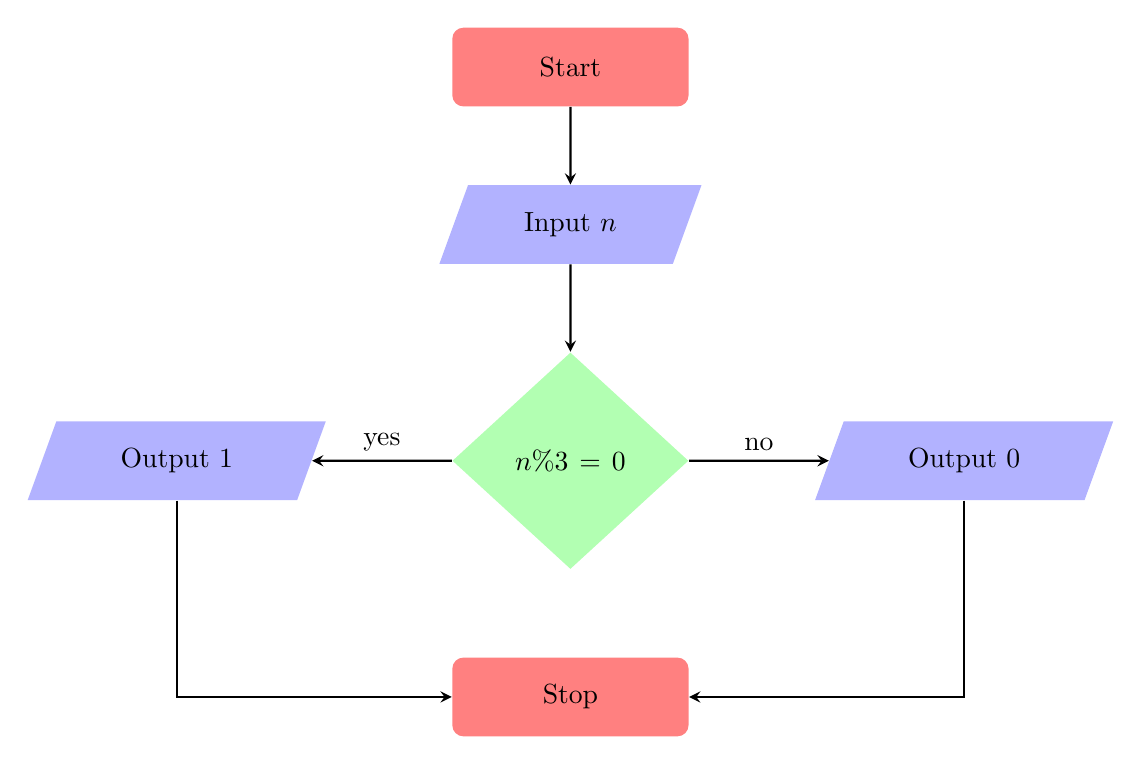
\begin{tikzpicture}
    \node [startstop] at (0,0) (start) {Start};
    \node [io] at (0,-2) (io1) {Input $n$};
    \node [decision] at (0,-5) (decision) {$n\%3=0$};
    \node [io] at (5,-5) (io2) {Output 0};
    \node [io] at (-5,-5) (io3) {Output 1};
    \node [startstop] at (0,-8) (stop) {Stop};
    \draw [arrow] (start) -- (io1);
    \draw [arrow] (io1) -- (decision);
    \draw [arrow] (decision) -- node[anchor=south] {no}(io2);
    \draw [arrow] (decision) -- node[anchor=south] {yes} (io3);
    \draw [arrow] (io2) |- (stop);
    \draw [arrow] (io3) |- (stop);
    \end{tikzpicture}
\end{center}

Here is an example of an algorithm that solves the linear equation $Ax+B=C$ for $x$ if $A$, $B$, and $C$ are real numbers with $A\neq 0$. (Why do we need to assume that $A\neq 0$?)

\begin{center}
    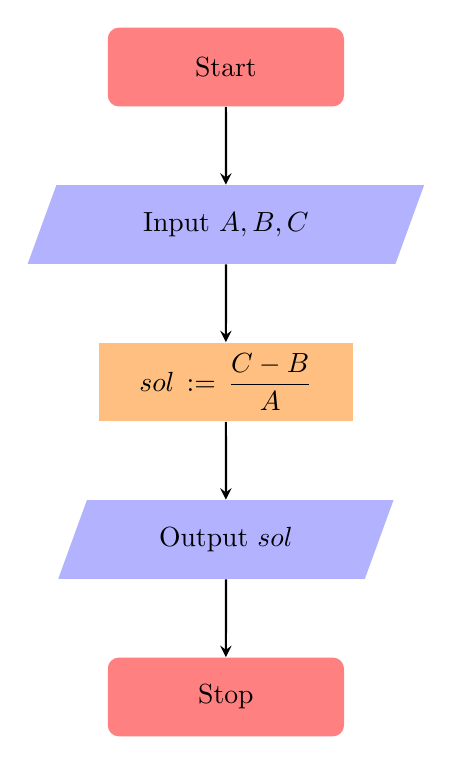
\begin{tikzpicture}
    \node [startstop] at (0,0) (start) {Start};
    \node [io] at (0,-2) (io1) {Input $A,B,C$};
    \node [process] at (0,-4) (process) {$sol:=\displaystyle \frac{C-B}{A}$};
    \node [io] at (0,-6) (io2) {Output $sol$};
    \node [startstop] at (0,-8) (stop) {Stop};
    \draw [arrow] (start) -- (io1);
    \draw [arrow] (io1) -- (process);
    \draw [arrow] (process) -- (io2);
    \draw [arrow] (io2) -- (stop);
    \end{tikzpicture}
\end{center}

The following examples illustrate a concept we will see over and over again. These flowcharts will have a loop showing that a certain step may be repeated multiple times until some condition is met.

Here is an example of an algorithm that finds the smallest integer greater than or equal to a real number $x\geq 0$.

\begin{center}
    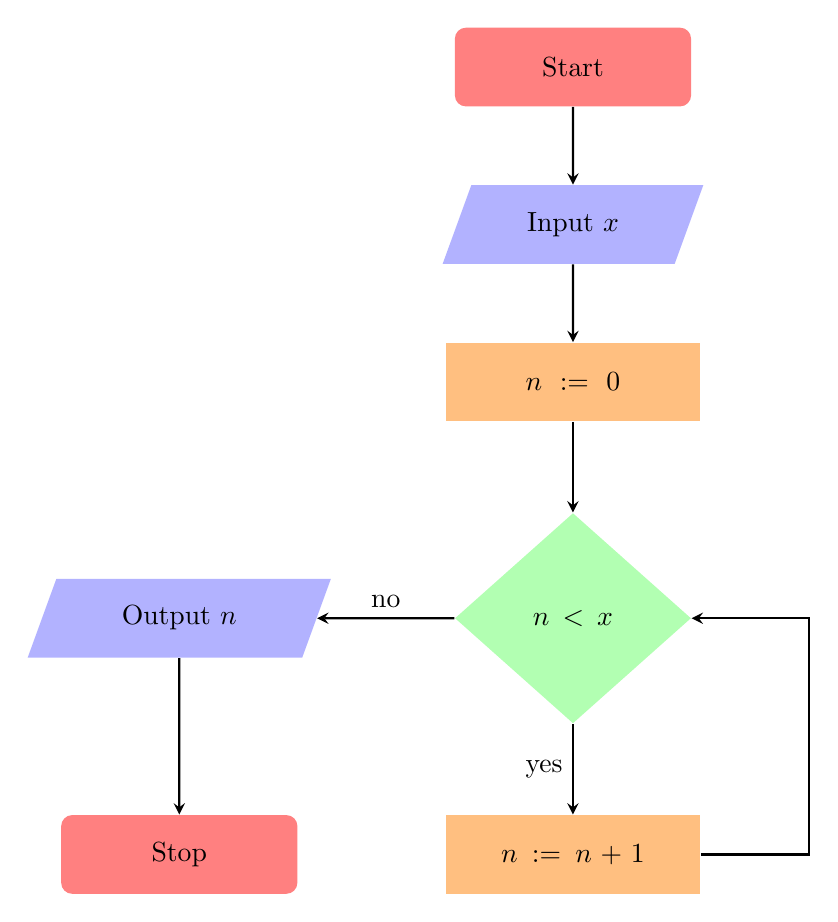
\begin{tikzpicture}
    \node [startstop] at (0,0) (start) {Start};
    \node [io] at (0,-2) (io1) {Input $x$};
    \node [process] at (0,-4) (process1) {$n:=0$};
    \node [decision] at (0,-7) (decision) {$n<x$};
    \node [io] at (-5,-7) (io2) {Output $n$};
    \node [process] at (0,-10) (process2) {$n:=n+1$};
    \node [startstop] at (-5,-10) (stop) {Stop};

    \draw [arrow] (start) -- (io1);
    \draw [arrow] (io1) -- (process1);
    \draw [arrow] (process1) -- (decision);
    \draw [arrow] (decision) -- node[anchor=east] {yes} (process2);
    \draw [arrow] (decision) -- node[anchor=south] {no} (io2);
    \draw [arrow] (io2) -- (stop);
    \draw [arrow] (process2) -- (3,-10) |- (decision);
    \end{tikzpicture}
\end{center}

Here is an example of an algorithm that computes the sum $1+2+3+\cdots+n$ for any integer $n>0$.

\begin{center}
    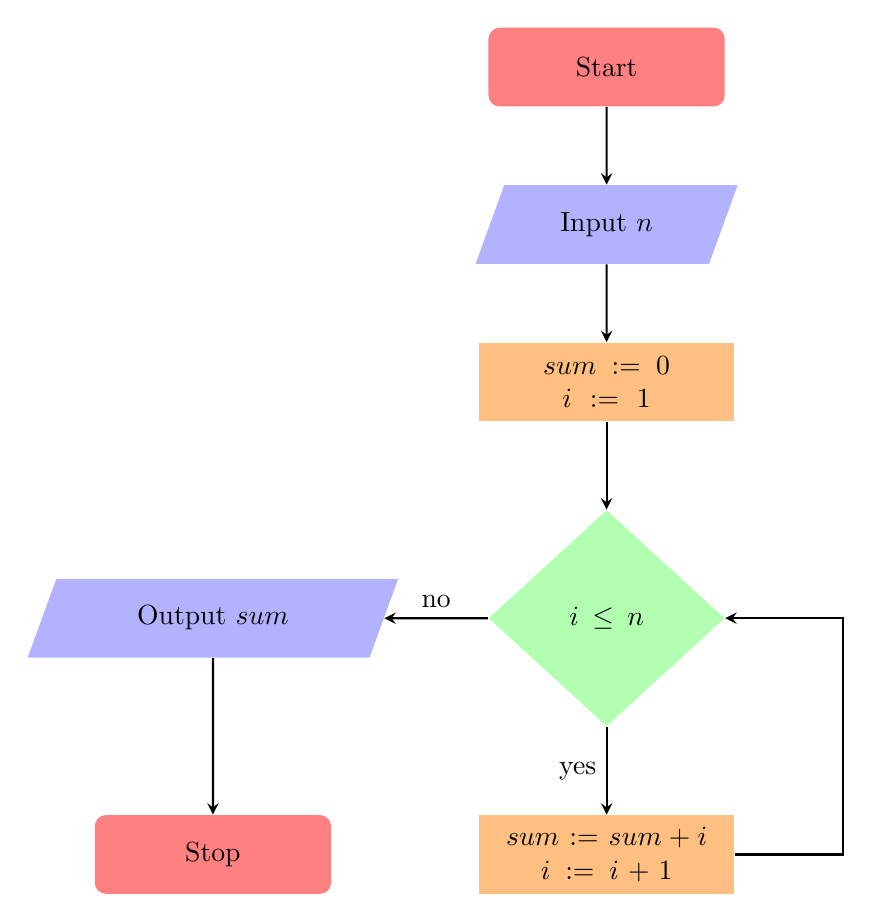
\begin{tikzpicture}
    \node [startstop] at (0,0) (start) {Start};
    \node [io] at (0,-2) (io1) {Input $n$};
    \node [process] at (0,-4) (process1) {$sum:=0$\\$i:=1$};
    \node [decision] at (0,-7) (decision) {$i\leq n$};
    \node [io] at (-5,-7) (io2) {Output $sum$};
    \node [process] at (0,-10) (process2) {$sum:=sum+i$\\$i:=i+1$};
    \node [startstop] at (-5,-10) (stop) {Stop};

    \draw [arrow] (start) -- (io1);
    \draw [arrow] (io1) -- (process1);
    \draw [arrow] (process1) -- (decision);
    \draw [arrow] (decision) -- node[anchor=east] {yes} (process2);
    \draw [arrow] (decision) -- node[anchor=south] {no} (io2);
    \draw [arrow] (io2) -- (stop);
    \draw [arrow] (process2) -- (3,-10) |- (decision);
    \end{tikzpicture}
\end{center}

In the example above we need to track two quantities. The value of \verb|i| tracks the number of times we go through the loop and while \verb|sum| is updated after each iteration appropriately until we reach the desired sum. Note that the order of the instructions when updating \verb|i| and \verb|sum| is important. (Why?)

Here is an example of an algorithm that computes the number of integers divisible by 6 in the interval $[1,n]$ for some integer $n>0$.

\begin{center}
    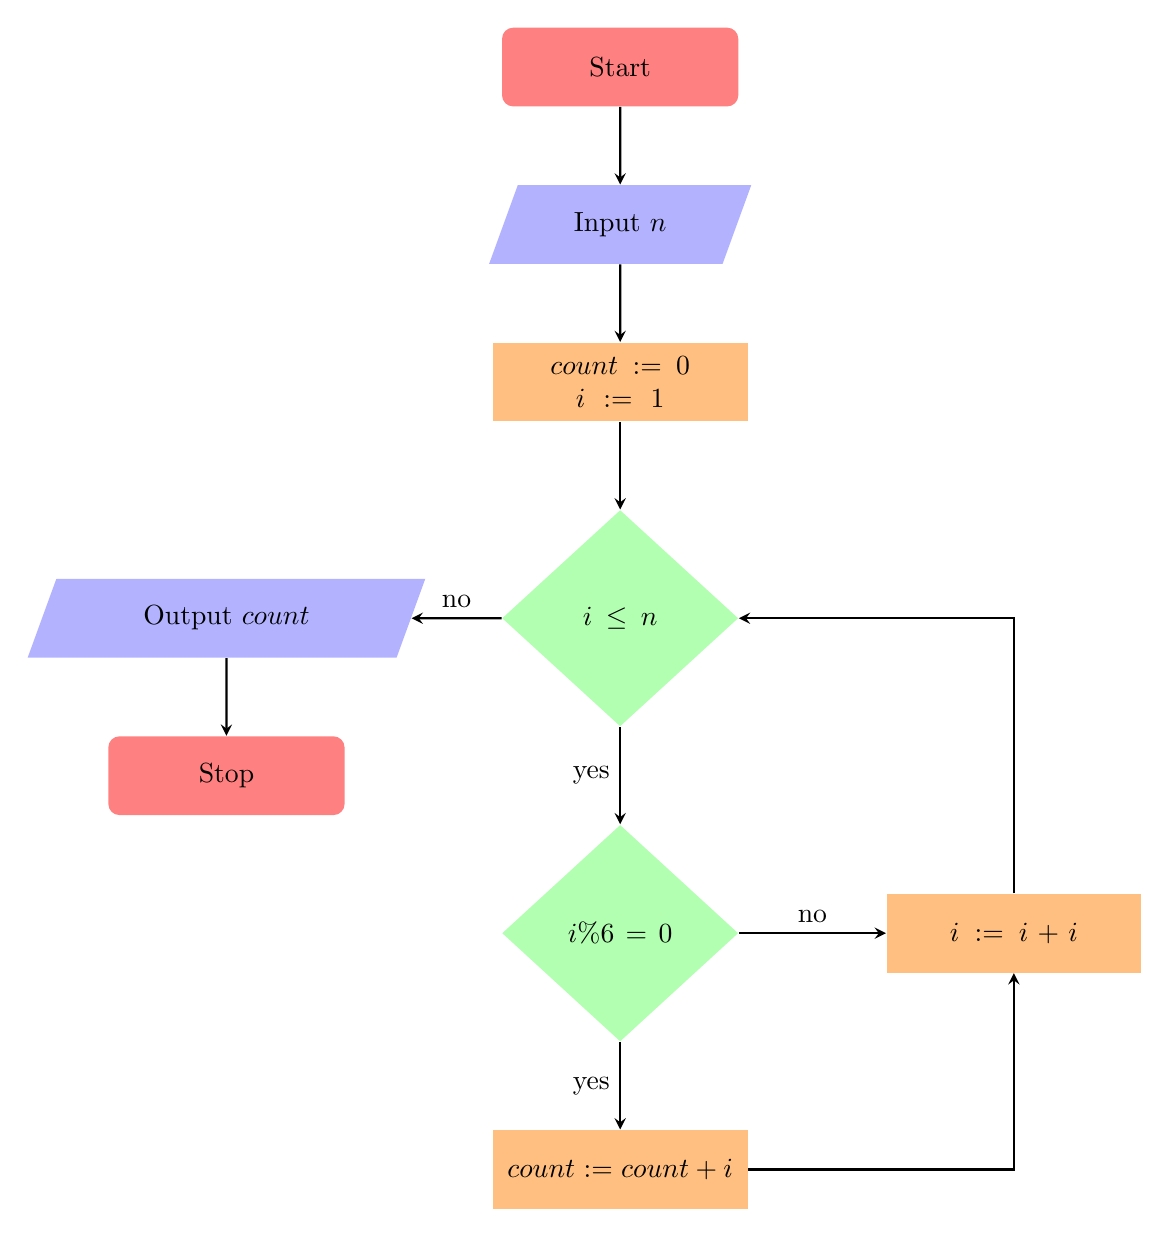
\begin{tikzpicture}
    \node [startstop] at (0,0) (start) {Start};
    \node [io] at (0,-2) (io1) {Input $n$};
    \node [process] at (0,-4) (process1) {$count:=0$\\$i:=1$};
    \node [decision] at (0,-7) (decision1) {$i\leq n$};
    \node [decision] at (0,-11) (decision2) {$i\%6=0$};
    \node [io] at (-5,-7) (io2) {Output $count$};
    \node [process] at (0,-14) (process2) {$count:=count+i$};
    \node [process] at (5,-11) (process3) {$i:=i+i$};
    \node [startstop] at (-5,-9) (stop) {Stop};

    \draw [arrow] (start) -- (io1);
    \draw [arrow] (io1) -- (process1);
    \draw [arrow] (process1) -- (decision1);
    \draw [arrow] (decision1) -- node[anchor=east] {yes} (decision2);
    \draw [arrow] (decision1) -- node[anchor=south] {no} (io2);
    \draw [arrow] (decision2) -- node[anchor=east] {yes} (process2);
    \draw [arrow] (decision2) -- node[anchor=south] {no} (process3);
    \draw [arrow] (io2) -- (stop);
    \draw [arrow] (process2) -| (process3);
    \draw [arrow] (process3) |- (decision1);
    \end{tikzpicture}
\end{center}

In the example above we also track two quantities. Notice that in this case we have an additional decision compartment as we only update the count of numbers divisible by 6 when the current number under consideration, \verb|i|, is divisible by 6. Regardless of whether or not we update \verb|count|, we always increase the value of \verb|i| before looping back.

\section{Problems}

\begin{question}
	Develop an algorithm that takes in three real numbers $a$, $b$, and $c$ with $a\neq 0$ and determines if the roots of quadratic polynomial $ax^2+bx+c$ are real or not. If the roots are real, the output should be a 1. If the roots are complex, the output should be 0. Draw a flowchart for your algorithm.
	\begin{hint}
		Consider the quantity $b^2-4ac$. Note that the second hint for this problem is the solution.
	\end{hint}
	
	\begin{hint}
		\begin{center}
			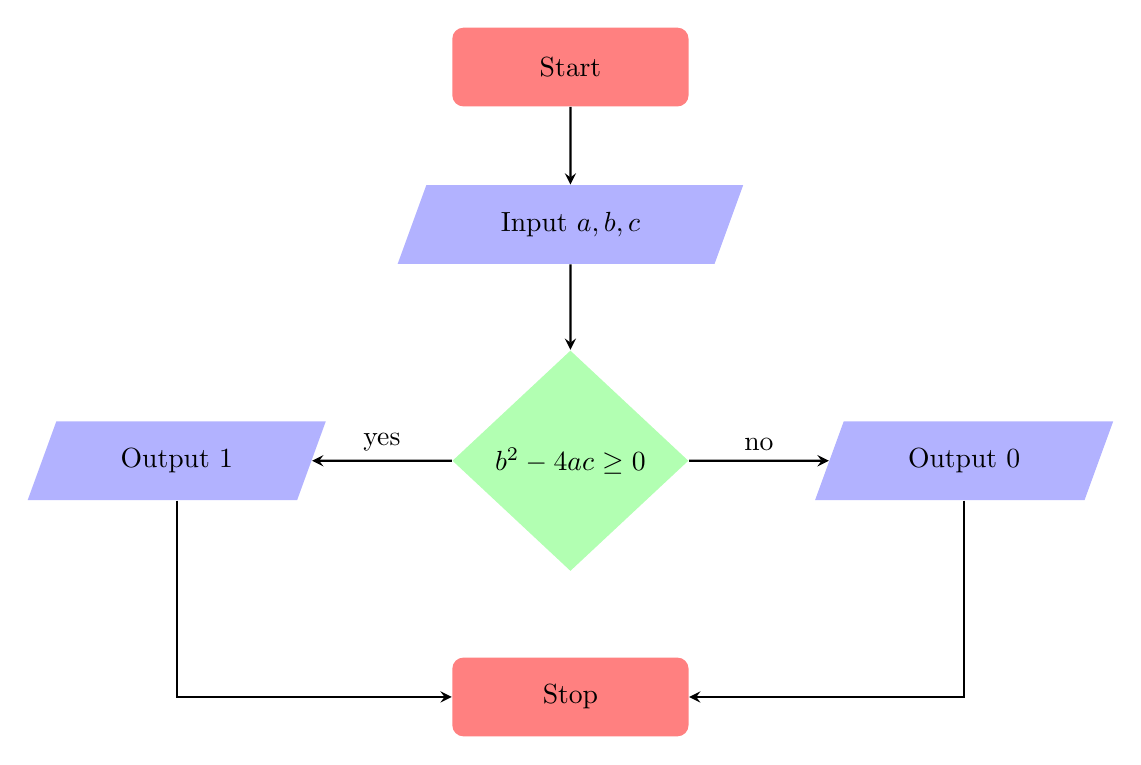
\begin{tikzpicture}
            \node [startstop] at (0,0) (start) {Start};
            \node [io] at (0,-2) (io1) {Input $a,b,c$};
            \node [decision] at (0,-5) (decision) {$b^2-4ac\geq 0$};
            \node [io] at (5,-5) (io2) {Output 0};
            \node [io] at (-5,-5) (io3) {Output 1};
            \node [startstop] at (0,-8) (stop) {Stop};
            \draw [arrow] (start) -- (io1);
            \draw [arrow] (io1) -- (decision);
            \draw [arrow] (decision) -- node[anchor=south] {no}(io2);
            \draw [arrow] (decision) -- node[anchor=south] {yes} (io3);
            \draw [arrow] (io2) |- (stop);
            \draw [arrow] (io3) |- (stop);
            \end{tikzpicture}
		\end{center}
	\end{hint}
\end{question}

\begin{question}
	Develop an algorithm that takes in a positive integer $n$ and outputs ``Fizz" if the number is divisible only by 3 (and not 5), ``Buzz" if the number is divisible by 5 (and not 3), ``FizzBuzz" if the number is divisible by 15, and n otherwise. Draw a flowchart for your algorithm.
	\begin{hint}
		Consider determining if the number is divisible by 15 first. If it is not, then you can determine if it is divisible by just 3 or just 5. Note that the second hint for this problem is the solution.
	\end{hint}
	\begin{hint}
		\begin{center}
			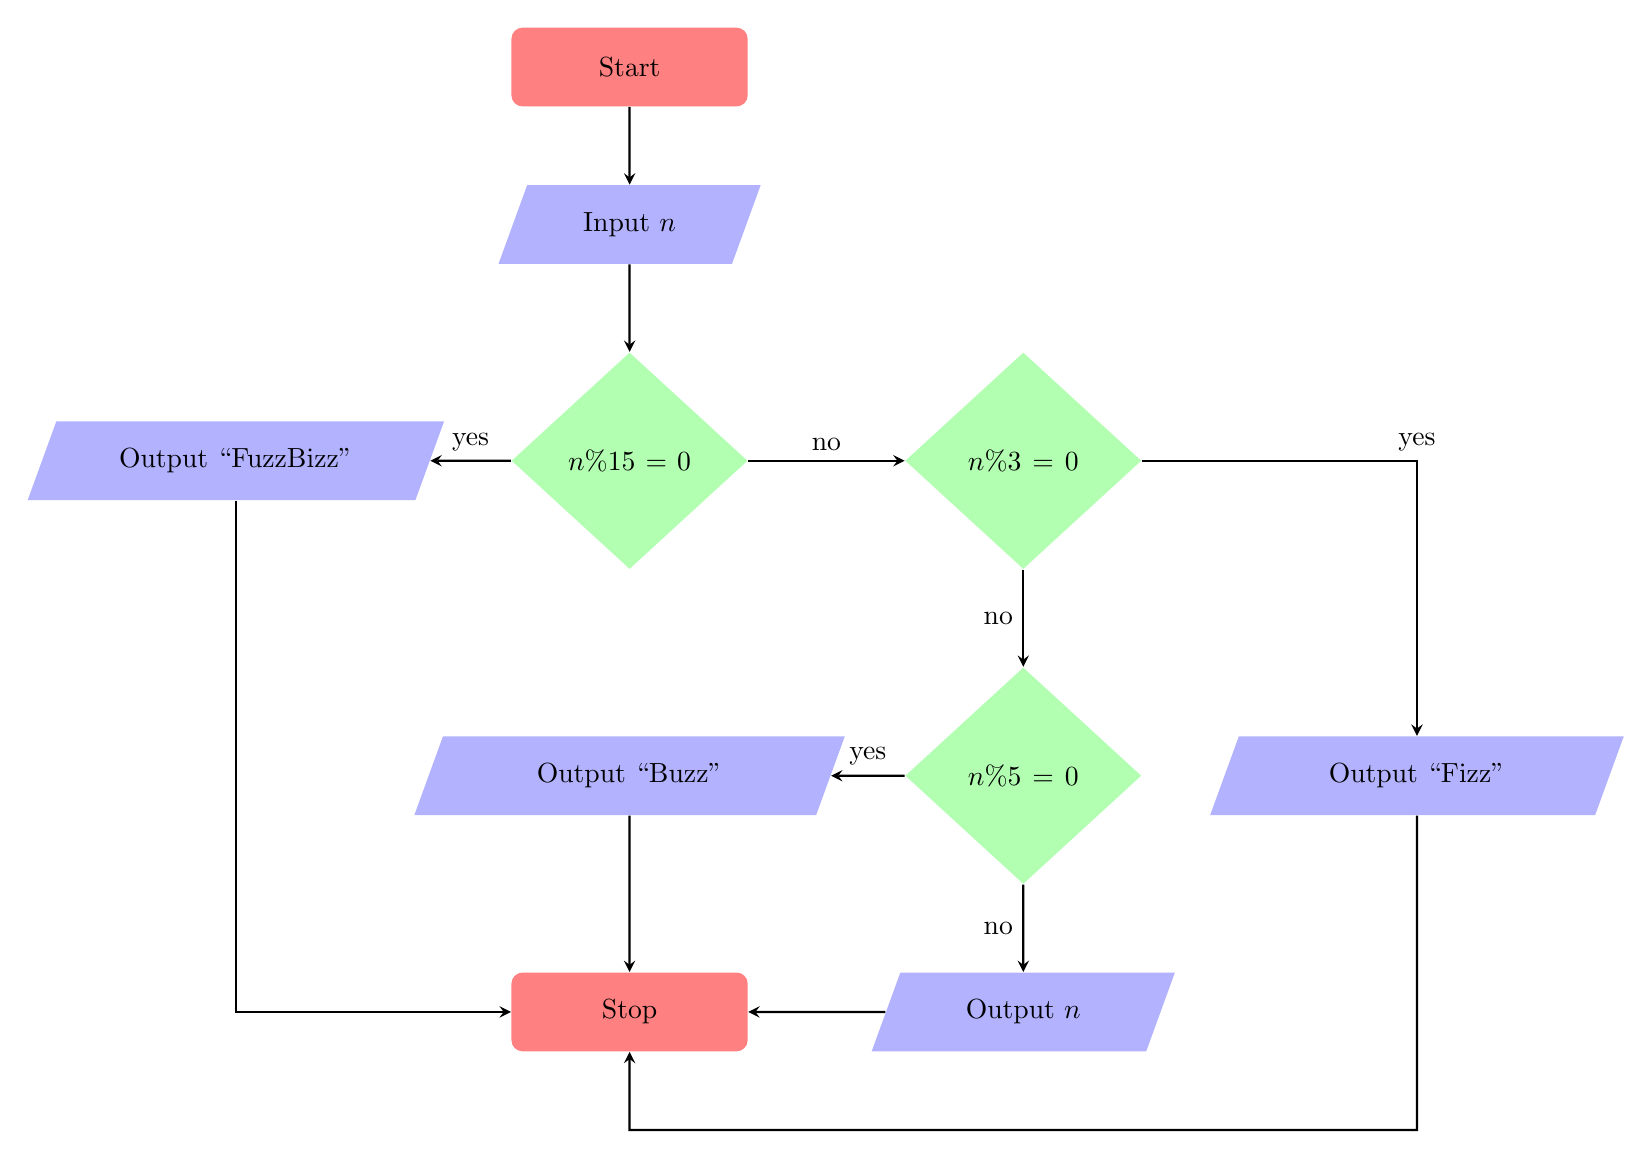
\begin{tikzpicture}
            \node [startstop] at (0,0) (start) {Start};
            \node [io] at (0,-2) (io1) {Input $n$};
            \node [io, label=center:Output ``FuzzBizz"] at (-5,-5) (io2) {\phantom{Output ``Bizz"}};
            \node [decision] at (0,-5) (decision1) {$n\%15=0$};
            \node [decision] at (5,-5) (decision2) {$n\%3=0$};
            \node [io] at (0,-9) (io3) {Output ``Buzz"};
            \node [decision] at (5,-9) (decision3) {$n\%5=0$};
            \node [io] at (10,-9) (io4) {Output ``Fizz"};
            \node [startstop] at (0,-12) (stop) {Stop};
            \node [io] at (5,-12) (io5) {Output $n$};

            \draw [arrow] (start) -- (io1);
            \draw [arrow] (io1) -- (decision1);
            \draw [arrow] (decision1) -- node[anchor=south] {yes}(io2);
            \draw [arrow] (decision1) -- node[anchor=south] {no} (decision2);
            \draw [arrow] (decision2) -| node[anchor=south] {yes} (io4);
            \draw [arrow] (decision2) -- node[anchor=east] {no} (decision3);
            \draw [arrow] (decision3) -- node[anchor=south] {yes} (io3);
            \draw [arrow] (decision3) -- node[anchor=east] {no} (io5);
            \draw [arrow] (io2) |- (stop);
            \draw [arrow] (io3) -- (stop);
            \draw [arrow] (io4) -- (10,-13.5) -| (stop);
            \draw [arrow] (io5) -- (stop);
            \end{tikzpicture}
		\end{center}
	\end{hint}
\end{question}

\begin{question}
	The factorial function is defined for a nonnegative integer $n$ in the following way:
	$$n! = \begin{cases}n(n-1)(n-2)\cdots 2\cdot 1 & \text{ if $n>0$,}\\
		1 & \text{ if $n=0$.}
	\end{cases}$$
	Develop an algorithm for computing $n!$ and draw a flowchart for your algorithm.
	\begin{hint}
		This problem is similar to the example above where you wanted to compute $1+2+\cdots+n$. Note that the second hint for this problem is the solution.
	\end{hint}
	\begin{hint}
		\begin{center}
			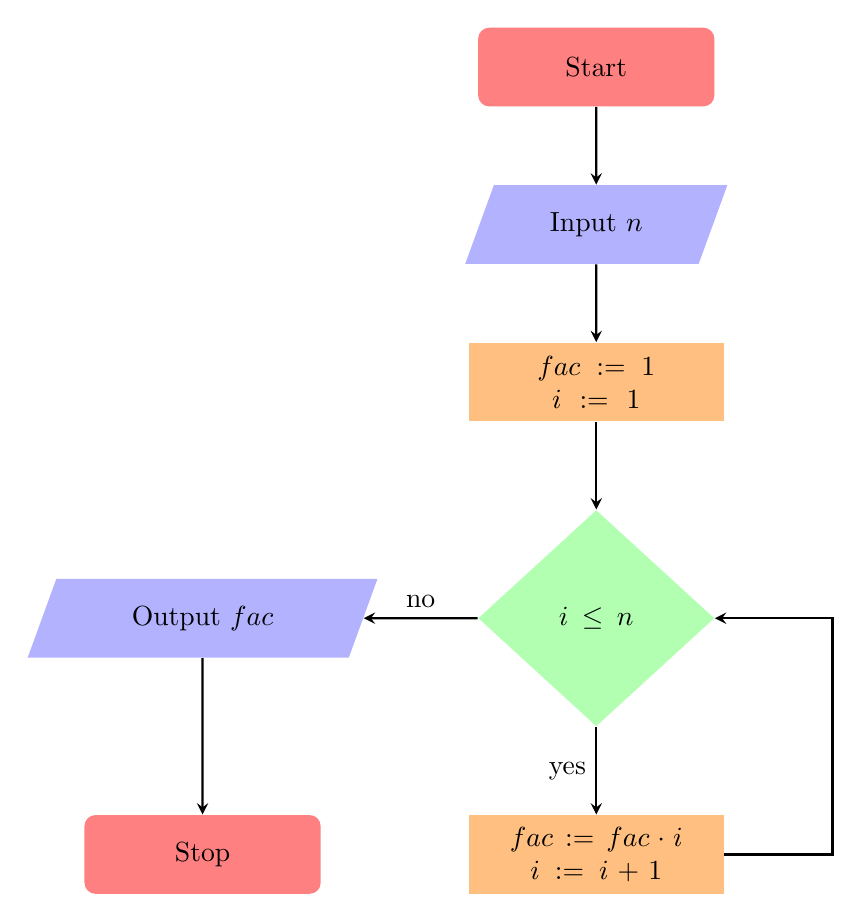
\begin{tikzpicture}
            \node [startstop] at (0,0) (start) {Start};
            \node [io] at (0,-2) (io1) {Input $n$};
            \node [process] at (0,-4) (process1) {$fac:=1$\\$i:=1$};
            \node [decision] at (0,-7) (decision) {$i\leq n$};
            \node [io] at (-5,-7) (io2) {Output $fac$};
            \node [process] at (0,-10) (process2) {$fac:=fac\cdot i$\\$i:=i+1$};
            \node [startstop] at (-5,-10) (stop) {Stop};

            \draw [arrow] (start) -- (io1);
            \draw [arrow] (io1) -- (process1);
            \draw [arrow] (process1) -- (decision);
            \draw [arrow] (decision) -- node[anchor=east] {yes} (process2);
            \draw [arrow] (decision) -- node[anchor=south] {no} (io2);
            \draw [arrow] (io2) -- (stop);
            \draw [arrow] (process2) -- (3,-10) |- (decision);
            \end{tikzpicture}
		\end{center}
	\end{hint}
\end{question}

For the next few problems we will need the following definition:

\begin{definition}
	For a nonzero integer $n$, we say that a nonzero integer $m$ is a divisor if and only if there is no remainder when dividing $n$ by $m$.
\end{definition}

For example, 2 is a divisor of 10, but 3 is not a divisor of 10.

\begin{question}
	Develop an algorithm that takes in two nonzero integers $m$ and $n$ and determines if $m$ is a divisor of $n$. If $m$ is a divisor of $n$, the output should be 1. If $m$ is not a divisor of $n$, the output should be 0. Draw a flowchart for your algorithm.
	\begin{hint}
		The solution to this problem is similar to the example above that determines if a number is divisible by 3. The main difference is that 3 should be replaced by the additional input $m$. Note that the second hint for this problem is the solution.
	\end{hint}
	\begin{hint}
		\begin{center}
			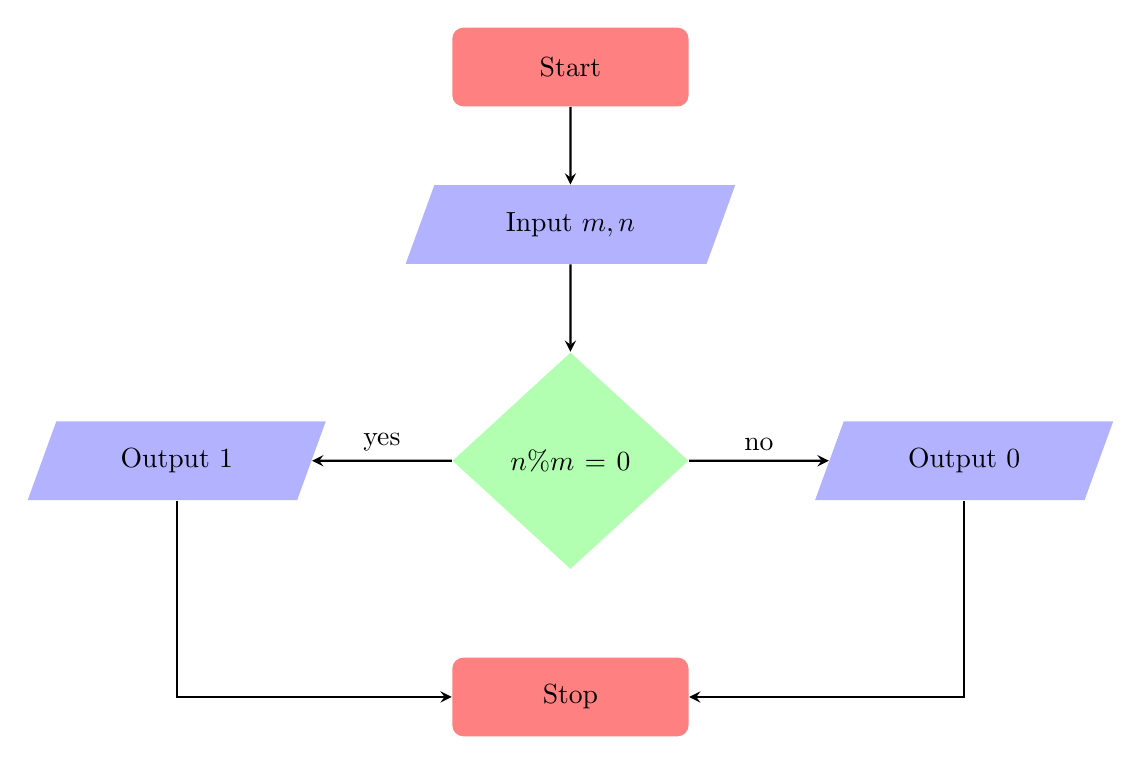
\begin{tikzpicture}
            \node [startstop] at (0,0) (start) {Start};
            \node [io] at (0,-2) (io1) {Input $m,n$};
            \node [decision] at (0,-5) (decision) {$n\%m = 0$};
            \node [io] at (5,-5) (io2) {Output 0};
            \node [io] at (-5,-5) (io3) {Output 1};
            \node [startstop] at (0,-8) (stop) {Stop};
            \draw [arrow] (start) -- (io1);
            \draw [arrow] (io1) -- (decision);
            \draw [arrow] (decision) -- node[anchor=south] {no}(io2);
            \draw [arrow] (decision) -- node[anchor=south] {yes} (io3);
            \draw [arrow] (io2) |- (stop);
            \draw [arrow] (io3) |- (stop);
            \end{tikzpicture}
		\end{center}
	\end{hint}
\end{question}

\begin{question}
	Develop an algorithm that counts the number of (positive) divisors of $n$ for any integer $n>0$.
	\begin{hint}
		The positive divisors of $n$ will have to be in the interval $[1,n]$. (Why?)
	\end{hint}
	\begin{hint}
		The solution to this problem is similar to the example above that counds the number of integers divisible by 6 in the interval $[1,n]$. The main difference is that you are now checking if $n$ (not \verb|i|) is divisible by any of the numbers in the interval $[1,n]$. Note that the third hint for this problem is the solution.
	\end{hint}

	\begin{hint}
		\begin{center}
			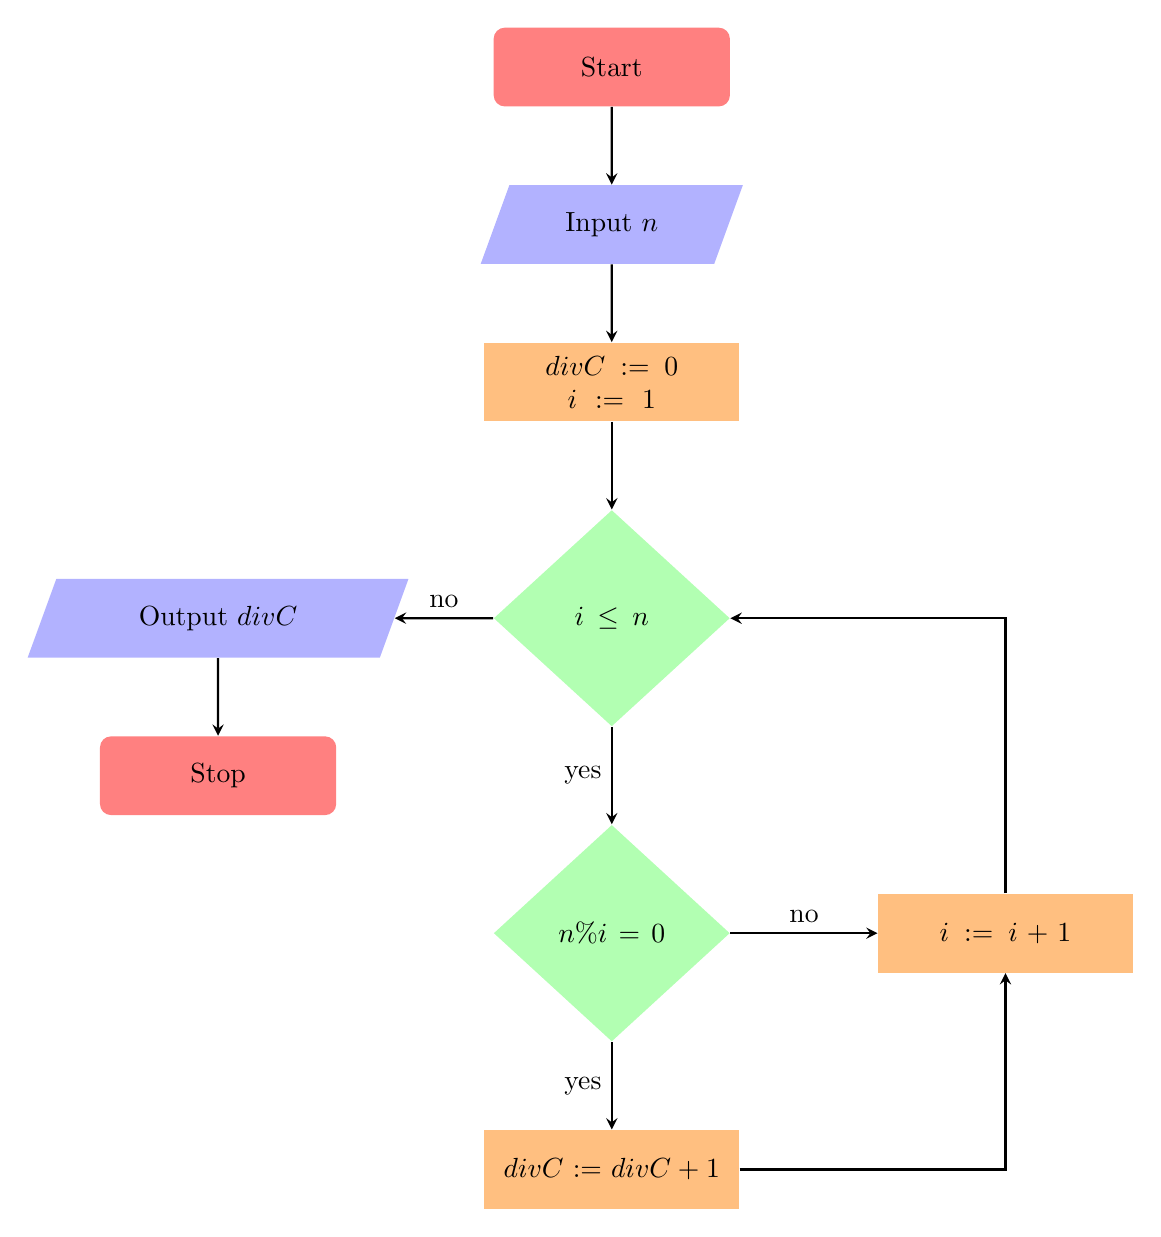
\begin{tikzpicture}
            \node [startstop] at (0,0) (start) {Start};
            \node [io] at (0,-2) (io1) {Input $n$};
            \node [process] at (0,-4) (process1) {$divC:=0$\\$i:=1$};
            \node [decision] at (0,-7) (decision1) {$i\leq n$};
            \node [decision] at (0,-11) (decision2) {$n\%i=0$};
            \node [io] at (-5,-7) (io2) {Output $divC$};
            \node [process] at (0,-14) (process2) {$divC:=divC+1$};
            \node [process] at (5,-11) (process3) {$i:=i+1$};
            \node [startstop] at (-5,-9) (stop) {Stop};

            \draw [arrow] (start) -- (io1);
            \draw [arrow] (io1) -- (process1);
            \draw [arrow] (process1) -- (decision1);
            \draw [arrow] (decision1) -- node[anchor=east] {yes} (decision2);
            \draw [arrow] (decision1) -- node[anchor=south] {no} (io2);
            \draw [arrow] (decision2) -- node[anchor=east] {yes} (process2);
            \draw [arrow] (decision2) -- node[anchor=south] {no} (process3);
            \draw [arrow] (io2) -- (stop);
            \draw [arrow] (process2) -| (process3);
            \draw [arrow] (process3) |- (decision1);
            \end{tikzpicture}
		\end{center}
	\end{hint}
\end{question}

\begin{question}
	Develop an algorithm that computes the sum of (positive) divisors of $n$ for any integer $n>0$.
	\begin{hint}
		The solution to this problem will use elements of the previous problem together with the example for how to compute $1+2+\cdots+n$. Note that the second hint for this problem is the solution.
	\end{hint}
	\begin{hint}
		\begin{center}
			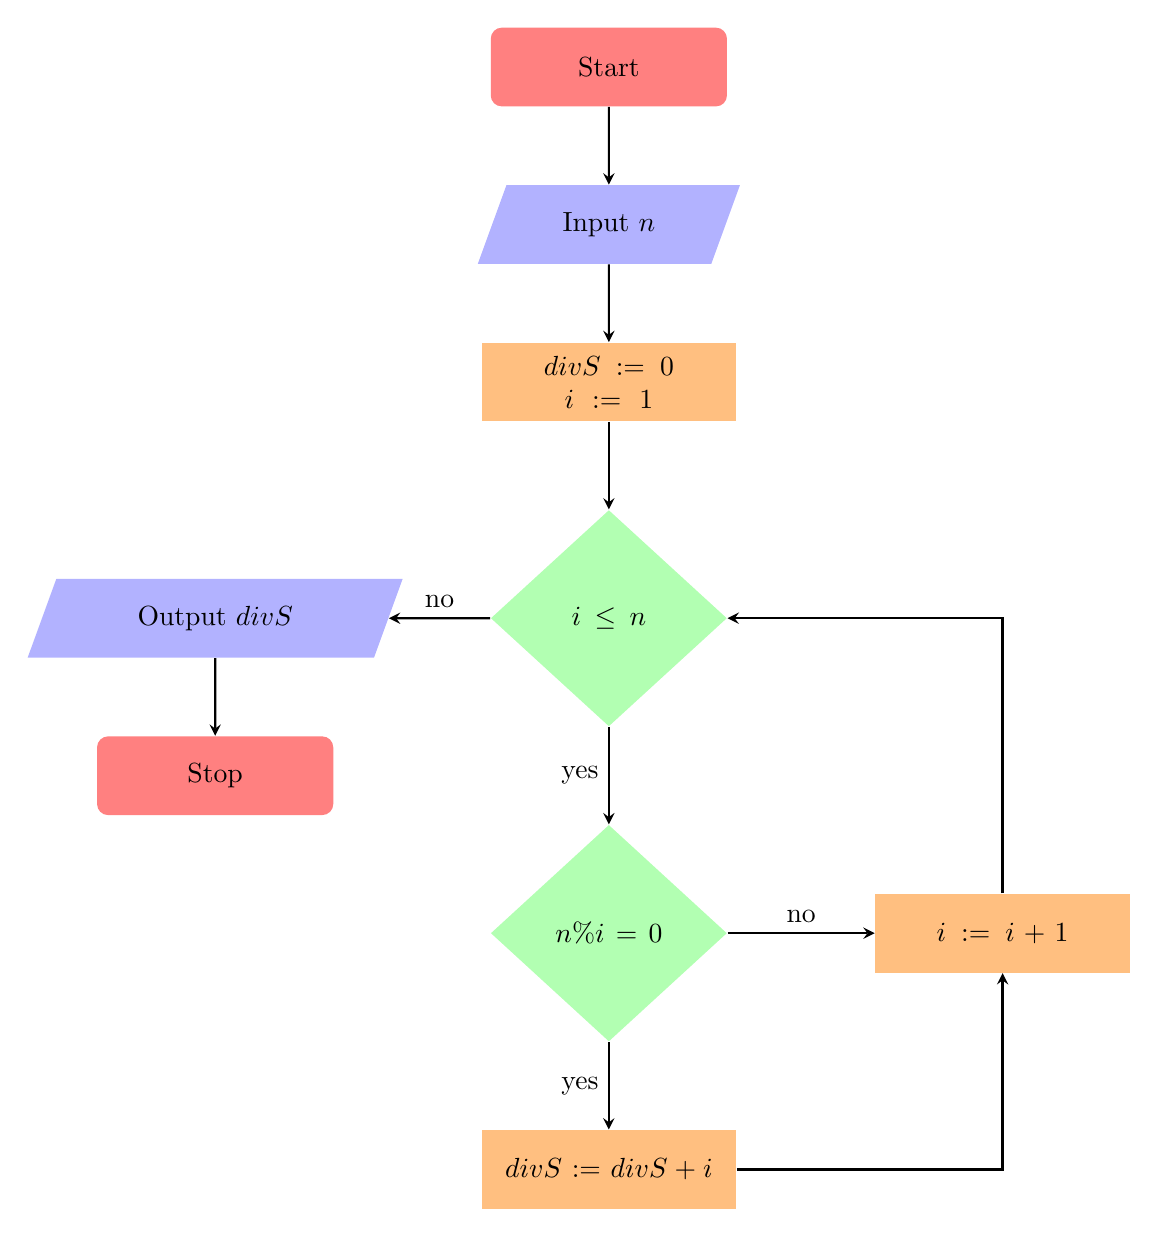
\begin{tikzpicture}
            \node [startstop] at (0,0) (start) {Start};
            \node [io] at (0,-2) (io1) {Input $n$};
            \node [process] at (0,-4) (process1) {$divS:=0$\\$i:=1$};
            \node [decision] at (0,-7) (decision1) {$i\leq n$};
            \node [decision] at (0,-11) (decision2) {$n\%i=0$};
            \node [io] at (-5,-7) (io2) {Output $divS$};
            \node [process] at (0,-14) (process2) {$divS:=divS+i$};
            \node [process] at (5,-11) (process3) {$i:=i+1$};
            \node [startstop] at (-5,-9) (stop) {Stop};

            \draw [arrow] (start) -- (io1);
            \draw [arrow] (io1) -- (process1);
            \draw [arrow] (process1) -- (decision1);
            \draw [arrow] (decision1) -- node[anchor=east] {yes} (decision2);
            \draw [arrow] (decision1) -- node[anchor=south] {no} (io2);
            \draw [arrow] (decision2) -- node[anchor=east] {yes} (process2);
            \draw [arrow] (decision2) -- node[anchor=south] {no} (process3);
            \draw [arrow] (io2) -- (stop);
            \draw [arrow] (process2) -| (process3);
            \draw [arrow] (process3) |- (decision1);
            \end{tikzpicture}
		\end{center}
	\end{hint}
\end{question}

\begin{question}
	 Prime numbers are integers greater than 1 that are not divisible by any positive integers other than 1 and hemselves. Develop an algorithm that determines if a positive integer $n$ is a prime number. If $n$ is a prime number, the output should be 1. If $n$ is not a prime number, the output should be 0. Draw a flowchart for your algorithm.
	\begin{hint}
		How many distinct divisors must primes have?
	\end{hint}
	\begin{hint}
		You should be able to modify the divisor count algorithm above by replacing the output with a decision compartment that determines whether the number is prime or not given its divisor count. Note that the third hint for this problem is the solution.
	\end{hint}
	\begin{hint}
		\begin{center}
			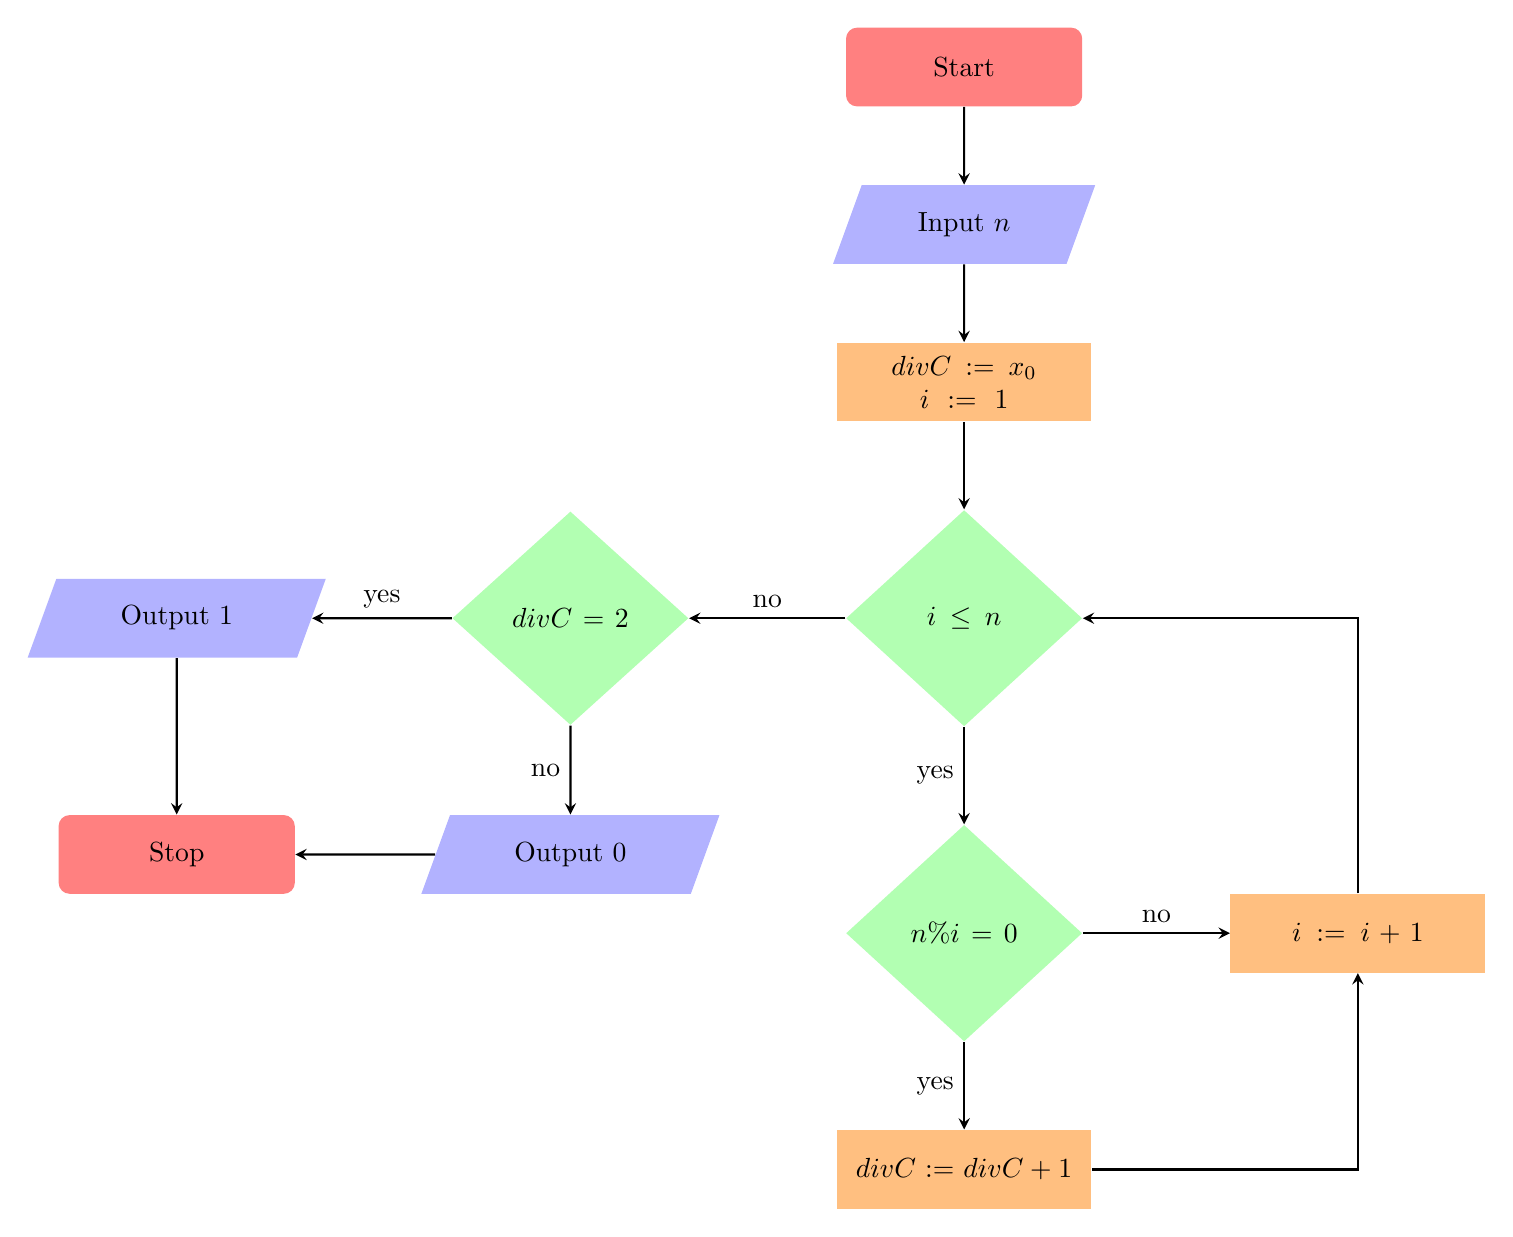
\begin{tikzpicture}
            \node [startstop] at (0,0) (start) {Start};
            \node [io] at (0,-2) (io1) {Input $n$};
            \node [process] at (0,-4) (process1) {$divC:=x_0$\\$i:=1$};
            \node [decision] at (0,-7) (decision1) {$i\leq n$};
            \node [decision] at (-5,-7) (decision2) {$divC=2$};
            \node [decision] at (0,-11) (decision3) {$n\%i=0$};
            \node [process] at (0,-14) (process2) {$divC:=divC+1$};
            \node [io] at (-5,-10) (io2) {Output 0};
            \node [io] at (-10,-7) (io3) {Output 1};
            \node [process] at (5,-11) (process3) {$i:=i+1$};
            \node [startstop] at (-10,-10) (stop) {Stop};

            \draw [arrow] (start) -- (io1);
            \draw [arrow] (io1) -- (process1);
            \draw [arrow] (process1) -- (decision1);
            \draw [arrow] (decision1) -- node[anchor=south] {no} (decision2);
            \draw [arrow] (decision2) -- node[anchor=east] {no} (io2);
            \draw [arrow] (decision1) -- node[anchor=east] {yes} (decision3);
            \draw [arrow] (decision2) -- node[anchor=south] {yes} (io3);
            \draw [arrow] (process2) -| (process3);
            \draw [arrow] (decision3) -- node[anchor=south] {no} (process3);
            \draw [arrow] (decision3) -- node[anchor=east] {yes} (process2);
            \draw [arrow] (process3) |- (decision1);
            \draw [arrow] (io2) -- (stop);
            \draw [arrow] (io3) -- (stop);
            \end{tikzpicture}
		\end{center}
	\end{hint}
\end{question}

\begin{question}
	Develop an algorithm that computes the largest integer less than or equal to a real number $x\geq 0$. Draw a flowchart for your algorithm.
	\begin{hint}
		The solution to this problem is similar to the example where you computed the smallest integer greater than or equal to a real number $x\geq 0$. Just be mindful of the output. Note that the second hint for this problem is the solution.
	\end{hint}
	\begin{hint}
		\begin{center}
			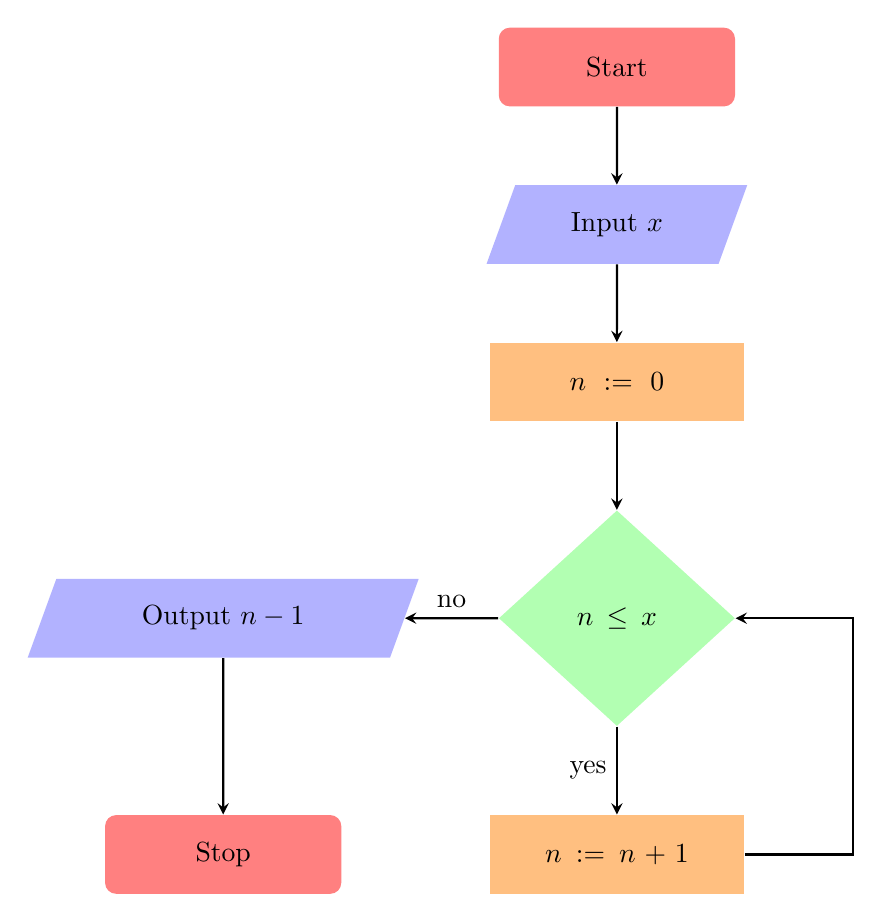
\begin{tikzpicture}
            \node [startstop] at (0,0) (start) {Start};
            \node [io] at (0,-2) (io1) {Input $x$};
            \node [process] at (0,-4) (process1) {$n:=0$};
            \node [decision] at (0,-7) (decision) {$n\leq x$};
            \node [io] at (-5,-7) (io2) {Output $n-1$};
            \node [process] at (0,-10) (process2) {$n:=n+1$};
            \node [startstop] at (-5,-10) (stop) {Stop};

            \draw [arrow] (start) -- (io1);
            \draw [arrow] (io1) -- (process1);
            \draw [arrow] (process1) -- (decision);
            \draw [arrow] (decision) -- node[anchor=east] {yes} (process2);
            \draw [arrow] (decision) -- node[anchor=south] {no} (io2);
            \draw [arrow] (io2) -- (stop);
            \draw [arrow] (process2) -- (3,-10) |- (decision);
            \end{tikzpicture}
		\end{center}
	\end{hint}
\end{question}

\begin{question}
	Develop an algorithm that computes the largest integer less than or equal to a real number $x<0$. Draw a flowchart for your algorithm.
	\begin{hint}
		Show that if $n$ is the largest integer less than or equal to a real number $x<0$, then $-n$ is the smallest integer greater than or equal to $-x$. Note that the second hint for this problem is the solution.
	\end{hint}
	\begin{hint}
		\begin{center}
			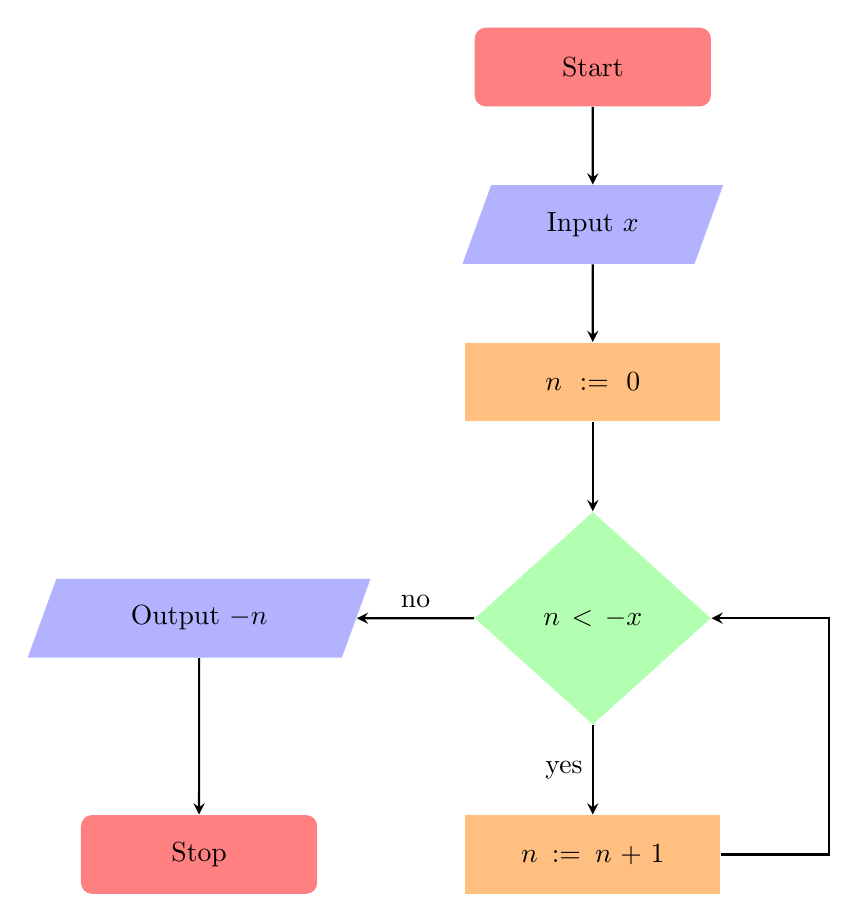
\begin{tikzpicture}
            \node [startstop] at (0,0) (start) {Start};
            \node [io] at (0,-2) (io1) {Input $x$};
            \node [process] at (0,-4) (process1) {$n:=0$};
            \node [decision] at (0,-7) (decision) {$n< -x$};
            \node [io] at (-5,-7) (io2) {Output $-n$};
            \node [process] at (0,-10) (process2) {$n:=n+1$};
            \node [startstop] at (-5,-10) (stop) {Stop};

            \draw [arrow] (start) -- (io1);
            \draw [arrow] (io1) -- (process1);
            \draw [arrow] (process1) -- (decision);
            \draw [arrow] (decision) -- node[anchor=east] {yes} (process2);
            \draw [arrow] (decision) -- node[anchor=south] {no} (io2);
            \draw [arrow] (io2) -- (stop);
            \draw [arrow] (process2) -- (3,-10) |- (decision);
            \end{tikzpicture}
		\end{center}
	\end{hint}
\end{question}

\begin{question}
	Develop an algorithm that computes the largest integer less than or equal to a real number $x$.
	\begin{hint}
		Combine the answers to the previous two problems. Note that the second hint for htis problem is the solution.
	\end{hint}
	\begin{hint}
		\begin{center}
			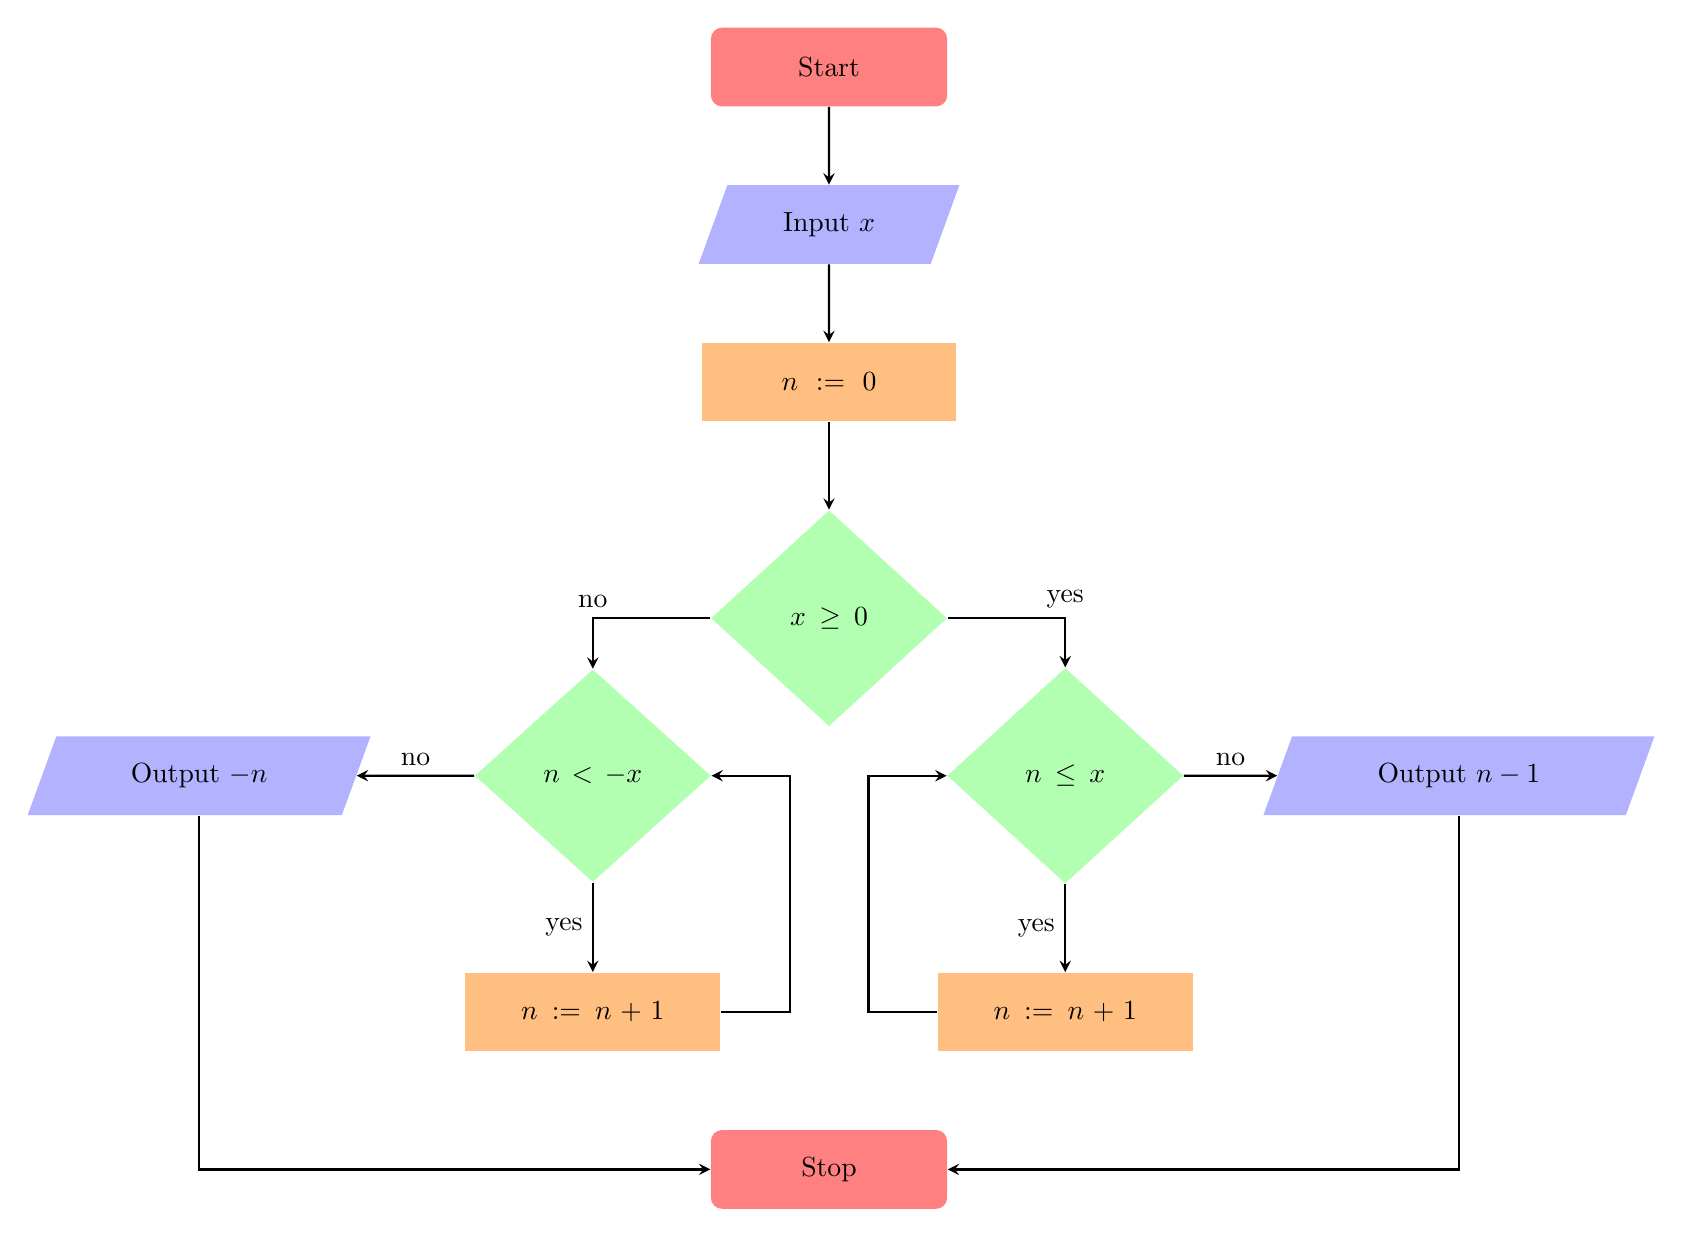
\begin{tikzpicture}
            \node [startstop] at (0,0) (start) {Start};
            \node [io] at (0,-2) (io1) {Input $x$};
            \node [process] at (0,-4) (process1) {$n:=0$};
            \node [decision] at (0,-7) (decision1) {$x\geq 0$};
            \node [decision] at (-3,-9) (decision2) {$n< -x$};
            \node [io] at (-8,-9) (io2) {Output $-n$};
            \node [process] at (-3,-12) (process2) {$n:=n+1$};
            \node [decision] at (3,-9) (decision3) {$n\leq x$};
            \node [io] at (8,-9) (io3) {Output $n-1$};
            \node [process] at (3,-12) (process3) {$n:=n+1$};
            \node [startstop] at (0,-14) (stop) {Stop};

            \draw [arrow] (start) -- (io1);
            \draw [arrow] (io1) -- (process1);
            \draw [arrow] (process1) -- (decision1);
            \draw [arrow] (decision1) -| node[anchor=south] {no} (decision2);
            \draw [arrow] (decision1) -| node[anchor=south] {yes} (decision3);
            \draw [arrow] (decision2) -- node[anchor=south] {no} (io2);
            \draw [arrow] (decision2) -- node[anchor=east] {yes}(process2);
            \draw [arrow] (process2) -- (-0.5,-12) |- (decision2);
            \draw [arrow] (io2) |- (stop);
            \draw [arrow] (decision3) -- node[anchor=south] {no} (io3);
            \draw [arrow] (decision3) -- node[anchor=east] {yes}(process3);
            \draw [arrow] (process3) -- (0.5,-12) |- (decision3);
            \draw [arrow] (io3) |- (stop);
            \end{tikzpicture}
		\end{center}
	\end{hint}
\end{question}

\end{document}
